%%% template.tex
%%%
%%% This LaTeX source document can be used as the basis for your technical
%%% paper or abstract.
%%%
%%% This example is tailored toward the two-page abstract. Please see "template.tex"
%%% for a more fully-annotated example.

\documentclass[review]{acmsiggraph}


% Load basic packages
\usepackage{balance}  % to better equalize the last page
\usepackage{graphics} % for EPS, load graphicx instead
\usepackage{times}    % comment if you want LaTeX's default font
\usepackage{url}      % llt: nicely formatted URLs

%\usepackage{compact_format}
\usepackage{customized_commands} % hongbo's customized commands
\graphicspath{
    {./Figures/}
    {./Images/}
    }


%%% Title of your article or abstract.

\title{Model-Guided 3D Sketching}

\author{}
\pdfauthor{}

%%% Used by the ``review'' variation; the online ID will be printed on
%%% every page of the content.

\TOGonlineid{45678}

% User-generated keywords.

\keywords{3d sketching, conceptual design, interface, canvas planes}

% With the "\setcopyright" command the appropriate rights management text will be added
% to your document.

%\setcopyright{none}
%\setcopyright{acmcopyright}
%\setcopyright{acmlicensed}
\setcopyright{rightsretained}
%\setcopyright{usgov}
%\setcopyright{usgovmixed}
%\setcopyright{cagov}
%\setcopyright{cagovmixed}
%\setcopyright{rightsretained}

% The year of publication in the "\copyrightyear" command.

\copyrightyear{2016}

%%% Conference information, from the completed rights management form.
%%% The "\conferenceinfo" command has two parameters:
%%%    - conference name
%%%    - conference date and location
%%% The "\isbn" field includes the year and month after the article ISBN.

%\conferenceinfo{SIGGRAPH 2016}{July 24-28, 2016, Anaheim, CA}
%\isbn{978-1-4503-ABCD-E/16/07}
%\doi{http://doi.acm.org/10.1145/9999997.9999999}

\begin{document}

%%% This is the ``teaser'' command, which puts an figure, centered, below
%%% the title and author information, and above the body of the content.

 \teaser{
   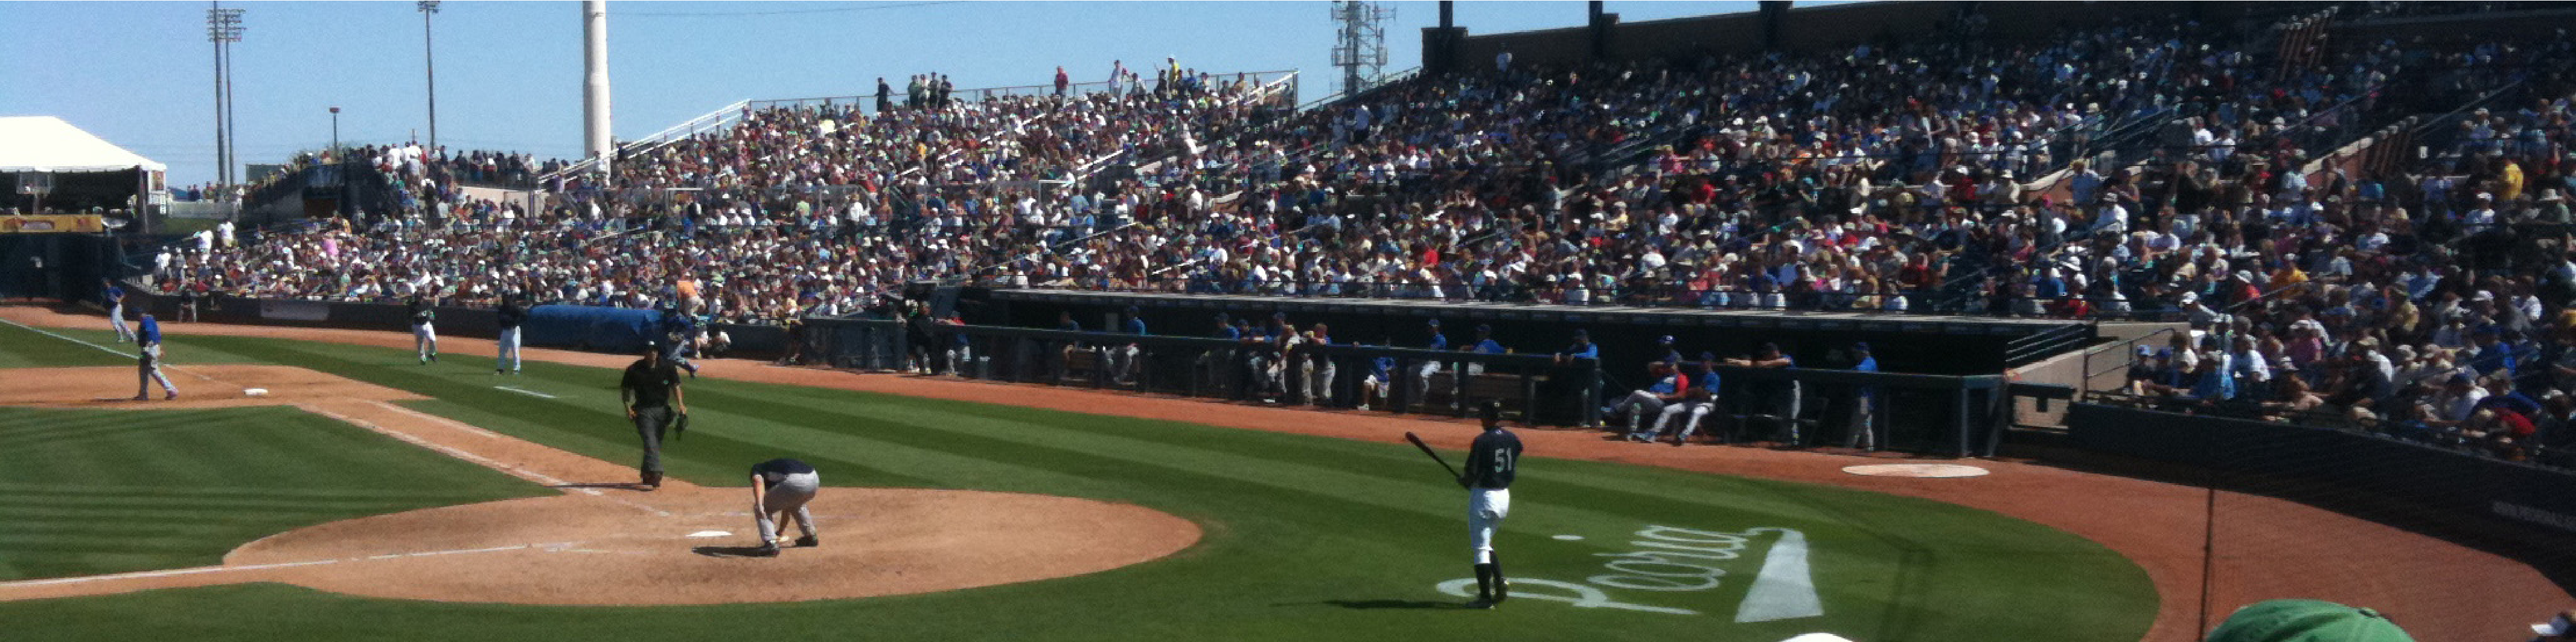
\includegraphics[height=1.5in]{images/sampleteaser}
   \caption{Spring Training 2009, Peoria, AZ.}
 }

\maketitle

\begin{abstract}


Abstract.

\end{abstract}

%
% The code below should be generated by the tool at
% http://dl.acm.org/ccs.cfm
% Please copy and paste the code instead of the example below.
%
\begin{CCSXML}
<ccs2012>
<concept>
<concept_id>10010147.10010371.10010382</concept_id>
<concept_desc>Computing methodologies~Image manipulation</concept_desc>
<concept_significance>500</concept_significance>
</concept>
<concept>
<concept_id>10010147.10010371.10010382.10010236</concept_id>
<concept_desc>Computing methodologies~Computational photography</concept_desc>
<concept_significance>300</concept_significance>
</concept>
</ccs2012>
\end{CCSXML}

\ccsdesc[500]{Computing methodologies~Image manipulation}
\ccsdesc[300]{Computing methodologies~Computational photography}

%
% End generated code
%

% The next three commands are required, and insert the user-generated keywords,
% The CCS concepts list, and the rights management text.
% Please make sure there is a blank line between each of these three commands.

\keywordlist

\conceptlist

\printcopyright

\section{Introduction}

% background: 3D sketching
Drawing a 2D sketch is often considered more intuitive and much faster than directly creating a 3D model. To facilitate 3D browsing of sketched objects, various 3D sketching systems \cite{dorsey2007mental,bae2008ilovesketch,Zheng2016}, which aim to lift 2D input sketches to 3D, have been proposed for early concept design. Most of the existing 3D sketching systems focus on 3D interpretation of 2D sketches alone, leading to a rather ill-posed problem. Additional assumptions or user inputs are thus often needed to resolve interpretation ambiguities.

We observe that designers often have to further develop ideas based on existing 3D models, which for example are intermediate models from an iterative design process. Designers may also start with an initial 3D model either retrieved from a shape repository (e.g., via a sketching interface \cite{Eitz:2012a}) or acquired by 3D-scanning a physical object for renovation \cite{Chen2015}. While the existing 3D sketching systems typically support the rendering of 3D sketches overlaid with a given 3D model, they either completely ignore or do not fully exploit the information of the 3D model for sketch interpretation. To the best of our knowledge, none of them is directly applicable to even simple examples shown in \ca{Figure~\ref{}}.



%Creating 3D models or scene is a fundamental task for many applications including games, movies, or real product design. This process requires well-trained artists to work on professional software with many iterations. In each iteration, the artists create a intermediate model and get feedback from their clients. Then they revise the intermediate model to produce a new version. The iteration ends until the clients satisfy the results. During this production process, the communication between the artists and the clients is crucial since a good communication may significantly reduce the production time.

%Communication through textural description is not sufficient since it may cause misunderstanding. A description with visual example is always preferable due to it is easy for understanding and with less mistakes during the communication. Since the intermediate results of the modeling is in 3D form, it would be better if the visual example is also 3D. However, most of the time the clients are not professionals of the modeling software, or even laymen of 3D modeling. In this case, it becomes challenging for the clients to create a 3D visual example to illustrate their requirement to the artists.

%Sketch is a simple and efficient media for expressing the idea. Almost anybody is able to draw an understandable sketch without training. Many 3D modeling or rendering softwares have provided sketching tools, such as grease pencil in Blender, to draw sketch in 3D. However, these tools are not easy to use since it still requires the user to carefully determine the 3D position of the sketch. Therefor they are still not a good choice for novice user.

In this work we will explore how a given 3D model can facilitate 3D interpretation of 2D sketches, and present a model-guided 3D sketching interface. We focus on sketching renovations of man-made objects or scenes, which often contain rich regular features, e.g., parallel lines, planar surfaces etc. A straightforward model-guided 3D sketching approach is to let users explicitly specify a planar surface of the model as a 3D canvas plane, on which 2D sketched strokes are projected to create 3D sketches. This approach often requires frequent changes of camera view due to the  visibility problem involved for plane selection. Worse, a 3D model typically has a small number of planar surfaces, significantly limiting the design space.

To address these problems we propose to perform a co-analysis of multiple 2D strokes, which are expected to lie in a single 3D plane. With our incremental interface a user draws strokes \emph{plane by plane},
but without explicit 3D plane specification. Once a group of 2D strokes constrained to a single plane is drawn, our inference engine automatically constructs a 3D plane by examining the attachment of those strokes to the 3D model and their correlation with the salient linear features of the model. With the constructed 3D plane, the 3D position of this group of 2D strokes can be easily determined.
\hongbo{TODO: additional assumption on the input strokes}

\todo{
suggestive interface; fix; rough strokes; for novice users;
annotation, renovation; 3D models, scenes;
%
It is easy and simple to use, so that it will be a suitable tool for novice user to express the idea of design.
}
% The surface is determined by our system automatically, based on the correlation between the strokes and the model. Since the drawn strokes may have multiple reasonable interpretations, there may exist several candidates of surfaces. We will provide a candidate list for the user to select.



\section{Related Work}
We are interested in inferring the depth of 2D strokes, which are typically sketched via graphic tablets. So the existing 3D sketching systems relying on special 3D input hardware (e.g., \cite{Sachs1991,Tsang2002}) is beyond the scope of our review here. 3D interpretation of 2D strokes is essentially an ill-posed problem and requires additional information to fix them in 3D. For example, a stroke might be required to drawn from multiple viewpoints \cite{Karpenko2004,bae2008ilovesketch,Rivers:2010}. % Kara:2007
In a single view, a stroke together with its shadow on a horizontal plane \cite{Cohen1999} or its symmetric counterpart \cite{bae2008ilovesketch} might be needed for 3D interpretation of this stroke. While these multi-curve approaches provide general ways to sketch 3D curves, they require accurate drawing, which is quite challenging (e.g., due to perceptual foreshortening biases).
%
% Our technique also take as input multiple strokes ...

A more common approach is to first specify a 3D sketch surface or canvas, on which 2D strokes can then be anchored one by one.
Various types of 3D sketch surface (e.g., planes, extruded surfaces~\cite{Tsang:2004,bae2008ilovesketch}, freeform surfaces~\cite{Kara2006,nealen2007fibermesh}, inflation surfaces~\cite{Grimm:2012}), have been explored for interactive 3D sketching. Among them 2D planes embedded in 3D (e.g., camera plane~\cite{bourguignon2001drawing}, parallel planes~\cite{dorsey2007mental}, co-axial planes~\cite{dorsey2007mental}, orthographic planes~\cite{Grossman2002,Tsang:2004,bae2008ilovesketch,Zheng2016}) are the most popular.
%
Such planes are often pre-configured and need to be explicitly activated (only one each time) before their use.
The planes might be translated and rotated in 3D for example using the traditional 3D object transformation tools.
%
Our work follows this line of research. However, we aim to automatically construct a 3D sketch plane by analyzing a group of 2D strokes lying on it and examining their relations to a 3D guidance model. We believe that our technique can reduce the efforts for mode switching, plane selection and manipulation, thus providing a smoother sketching experience.

The main problem of using a specific type of sketch surface is that the space of possible 3D curves is limited to those lying on such sketch surfaces. To address this problem, Schmidt et al.~\shortcite{schmidt2009analytic} proposed to first incrementally construct a linear 3D scaffold and then infer more freeform 3D curves from the scaffold. Our input 3D model for guidance is similar to their 3D scaffold in a sense that both of them provide geometric constraints (e.g., snapping{~\cite{bier1990snap}})
to filter the space of admissible 3D curves. Since the approach of Schmidt et al. incrementally fixes strokes in 3D \emph{one by one}, without using or forming any sketch canvas, it does not support casual sketching of 3D curves (\ca{Figure~\ref{}}), which cannot induce geometric constraints from the scaffold.

Face planarity is one of the fundamental geometric constraints used in automated interpretation of \emph{a complete sketch} (e.g.,~\cite{Lipson:1996,Chen:2008f,Zou2015}). Many existing works aim for the reconstruction of 3D polyhedra (with planar faces). Recently, Xu et al. \shortcite{xu2014true2form} present a mathematical framework to infer piecewise-smooth curve networks from 2D drawings. Such curve networks can be finally surfaced to create 3D surface models~\cite{Pan:2015}. Since 2D sketched strokes need to be ultimately mapped to 3D models to be reconstructed, these works all require relatively clean input drawings. Instead, our technique accepts more rough strokes as input and aim for rapid concept redesign of a given model.
%, similar to ~\cite{bourguignon2001drawing,dorsey2007mental,Zheng2016}.

Most of the above 3D sketching systems focus on the creation of 3D sketches from scratch, and only very few works explicitly discuss their use in the context of existing 3D models. Schmidt et al.~\shortcite{schmidt2009analytic} render 3D sketches overlaid with an existing 3D model, but do not exploit any model information for sketch interpretation. Bourguignon et al. \cite{bourguignon2001drawing} determine the depth of a canvas plane parallel to camera plane by examining the attachment of a stroke to a given 3D model. The \emph{OverCoat} technique~\cite{Schmid:2011} enables 3D painting by introducing isosurfaces of a proxy model as canvas. Similarly, \emph{SecondSkin} require strokes sketched on and around 3D geometry to build new layered structures. In contrast, we aim to automatically derive canvas planes from a given model to anchor 2D strokes, which are not necessarily on, around or attached to the model. 

3D sketching has also been studied in the context of single or multiple images. The existing approaches mainly use images as reference for 2D sketching, and employ the existing sketch interpretation techniques or their variations to fix 2D strokes in 3D (e.g., sketch planes adopted in~\cite{Tsang:2004,Paczkowski:2011}, modified Lipson optimization in~\cite{Lau:2010}). Very recently, Zheng et al.~\shortcite{Zheng2016}
proposed to first derive a 3D cuboid from a reference image (to align with respective vanishing directions) and then sweep out candidate canvas planes from the three orthogonal faces of the cuboid. Similar to ours, their technique then formulates sketch interpretation as a selection problem from a set of context-inducted canvas planes. While their system is rather powerful, it might take several hours for first-time users to get familiar with their system. This is largely due to excessive user intervention needed for camera calibration, relation annotation, stroke grouping, etc. We aim for an easy-to-use model-guided 3D sketching system by heavily exploiting the stroke-model relations to minimize user intervention. 

Due to the simplicity and intuitiveness, many sketch-based interfaces have been proposed for 3D modeling and editing (see an insightful survey in~\cite{olsen2009sketch}). A large category of existing techniques for sketch-based modeling from scratch are \emph{reconstruction-based} (e.g.,~\cite{Zeleznik:1996,Igarashi:1999,Karpenko:2006,nealen2007fibermesh}). They require accurate drawing, since the input strokes are somehow mapped directly to the output model. Sketching has been demonstrated powerful for editing existing shapes (e.g.,~\cite{singh1998wires,nealen:2005:sketch,Olsen:2005,Kara2006a}).
These approaches often use the existing models as sketch surfaces and aim for the generation of shape variations. Our goal is more similar to the retrieval-based approaches (e.g.,~\cite{Shin:2007,Lee:2008b,Xu:2013,Fan2013}), which intend to add new parts (models) into an existing model (scene) by retrieving the most similar parts (models) from a shape repository with respect to an input sketch as query. These approaches, however, are less interested in inferring 3D positions of the strokes, and after retrieval discard them, though sketches are often more expressive.
%







%\section{System Overview}
%
%%With the \ca{SKETCH} system, the user only needs to draw sketch over 3D model in a conventional 2D drawing manner: she does not needs to provide additional operation to specify the 3D information of the drawn sketch. Our system automatically bring the input 2D sketch to 3D based on the relation between the drawn strokes and the existing 3D features.
%
%\ca{1. brief introduction of the interface.}  The \ca{SKETCH} system adopts an incremental interface to construct a complete 3D sketch. The user draws the strokes plane by plane, i.e.,
%
%\ca{}

\section{User Interface}

%In this section we describe the interface of our sketching system.
Our prototype is composed of two windows: an input window for sketching and a preview window for displaying candidate 3{D} sketches, which are rendered in a specified view angle such that the user can easily perceive the results. Our user interface is then mainly devised into two interlaced stages: sketching and feedback. In the sketching stage, the user performs sketching on top of a 3{D} model on the screen. In a default mode, our system immediately returns 3{D} strokes for preview. Then, in the feedback stage, the user selectively confirms the current displayed results in 3{D} or override the results if she finds the default results not correct. To keep the sketching process smooth, we provide an intuitive feedback interface so as not to intervene the sketching process, which is necessary only when the current 3{D} content is falsely anchored.
%The operations in the preview window can also help to resolve the ambiguity introduced by the user's input.
%Each time the user draws strokes in the input window, the constructed 3D sketch is shown in the preview window in a carefully-chosen view angle to better express the 3D information of the resulting sketch.
In the following, we describe the interface for sketching and feedback in detail.

\subsection{Sketching}

%\ca{emphasis: our system follows the conventional sketching manner.}

To start with our system, the user first loads a 3{D} model which will be sketched over. This model is displayed in the input window with orthogonal projection, thus the 3D parallel relation is retained in the screen space. The view angle can be manipulated in \ca{the positioning mode} with rotation, translation, and zooming. When a desired view angle is obtained, the user can  enter \ca{the sketching mode} to draw sketch over the model. The drawing is performed using either mouse, digital pen, or a touch device, in a way similar to conventional drawing on paper. To convert the input strokes into 3D, we adopt an incremental strategy to reduce the potential ambiguities which arises with stroke number and let the user to resolve ambiguities when necessary. In particular, during the drawing, each time the user draws a set of strokes, before the feedback stage, we assume all the set of strokes lie on some planar canvas. Then, in a key stage, our system finds the planar canvas automatically by inferring its position and orientation from the relations between the drawn strokes and the model. Each time when the user draws a new stroke, this planar canvas will be updated. When the user finishes a set of strokes, she provides her feedback using the feedback interface (detailed in the Section \ref{sec:feedback}) to confirm the current set of 3{D} strokes and the drawn strokes will be converted into 3{D} by projecting them on the planar canvas. The user then continues to draw another set of strokes or manipulate the view angle. The user can also enter \ca{the erasing mode} to modify the previous drawn 3D strokes (see in the accompanying video).


\subsection{Feedback}\label{sec:feedback}
When the user draws strokes in the input window, our system automatically finds a default planar canvas and converts the drawn strokes into 3{D}. However, the 3{D} information of the sketch can not be perceived in the input window without changing the view angle. Therefore, we display the resulting 3{D} sketches in the preview window in a different view angle. In addition, since the user's input may have ambiguities, the potential planar canvas may not be unique. In this case, our algorithm also finds other possible candidate planar canvases and display the candidate planar canvases with the associated 3{D} sketches to the user in the preview window. The user, can select one from the candidate sketches, if the default one is not desired. To select the desired 3D sketch and associated canvas, the user simply use the stylus or finger to stroke across the desired candidate.  The user can also change the view angle to facilitate the selection process, if necessary. The selection mode and viewing mode can be switched by touching a floating button, which are displayed at the bottom of the preview window.

During the incremental sketching process, besides drawing strokes, an important task for the user to perform is to help confirm the current 3{D} contents and correct falsely estimated 3{D} strokes if exists. We find such interaction intuitive and typical as in traditional drawing system where a user often needs to confirm the current content using some emphatic means (e.g., by drawing heavy strokes over the contours of a character). To accomplish such task, a simple solution could be to include buttons on the task bar, such that the user could click these buttons to issue the desired commands. However, such interfaces often come with an additional travel distance cost as the user needs to move the mouse or finger from one place to another, frustrating the drawing process. Instead, we design a user-friendly interface for this task. We adopt floating buttons to minimize the stylus or finger movement when the user wants to issue a confirmation. During the drawing of a stroke, the buttons are invisible. When the stroke is finished, the floating buttons are shown next to the drawn strokes transparently. If the user continues to draw, the buttons fades away and will not introduce occlusion problem (see Figure \ref{} and the accompanying video for details).






%\ca{automatic view angle estimation}
%The view angle in the preview window is determined by the candidate 3D sketches. We choose a view angle such that the candidates

%\ca{manipulating view angle if necessary}


%\ca{canvas visualization??}

%\ca{selecting desired canvas}
%We have two

%\ca{mode switching by buttons in the bottom: window is small, no need to float}

%The user draws strokes in the input window, and the constructed candidate 3D sketches are shown in the preview window
% with a different view angle in which the difference of all candidate 3D sketches is




\section{Methodology}

%\ca{Brief idea: the relation between the strokes and projected model linear feature}
Our algorithm is based on an important observation: when people uses sketch to depict an additional part over a 3D model, some strokes behave like the structural part and usually share relations with the model. Therefore we can use the relations between the strokes and the model to estimate the 3D information of the drawn 2D strokes. 


\subsection{Relations between Shape and Strokes}


%\ca{pre processing of the shapes and strokes}
Before detecting the relations between the strokes and shape, we first extract straight segment from the drawn 2D strokes, and linear features from the shape. A straight segment is a consecutive part of stroke which is nearly straight. We use a simple growing algorithm to find the straight segments. Given a new stroke, we first uniformly resample it. The distance between sample points is \ca{10px} in our prototype. Then from the beginning of this resampled stroke, we add the points to current straight segment one by one, if the new added points will not introduce a sharp turning. Otherwise, current straight segment is finished and a new straight segment will be constructed. Then we filter out the short ones (less than \ca{50px}).

The linear features of the shape include sharp edge and main face normal. The sharp edges are extracted using a similar method in \ca{[Iwire]}. After extracting the sharp edges, we detect the straight ones similar to detecting the straight segment. The main face normal is obtained by first clustering the faces of the model with similar normal. The clustered faces forms several shape plane canvases. The normals of these canvases are considered as the linear feature of the shapes.

%\ca{relations: colinearity}
%
%\ca{relations: parallel}
After obtaining the straight segment of the stroke and linear feature of the shape, we detect the following relations:
\textbf{Colinearity.} This relation is detected between a straight segment and a straight sharp edge. The normals of shape plane canvases will not be used for detection since they miss position information.
\textbf{Parallel.} This relation is detected between a straight segment and a shape linear feature, including both straight sharp edge and normal of shape plane canvas.
These two relations are both detected in the screen space.

%\ca{relation: attachment, three level (corner, edge, face)}
Another important relation between the stroke and shape is \textbf{Attachment}. If a endpoint of the stroke is over or close to the shape, we consider that this endpoint attaches to the shape. To make the attachment more content-aware, the detection is performed in three levels. First, the attachment is detected between the endpoint and the corner of the shape. If no attachment relation is found, the detection continues between the endpoint and the sharp edges. If no attachment relation is found in this level, we then detect the attachment between the endpoint and the shape's face.


\subsection{Canvas Estimation}

The canvas is obtained from the relations between shape and strokes. Due to the ambiguity of the input, some of the detected relations are actually undesired. Therefore it is not wise to find a canvas which tries to fulfill all the detected relations. One observation is that, although the user's input contains ambiguity, most of the relations should be able to comply with each other, if the correct canvas is found. Motivated by this observation, we propose a two step approach to estimate the canvas.

First, we construct candidate canvases. Candidate canvases are all possible canvases which could be obtained by the combination of the relations. We found that the following combinations are able to yield valid canvases.

\textbf{Two colinearity.} If the corresponding two straight sharp edges could spans a plane, this combination can yield a valid canvas.

\textbf{One colinearity + one parallel.} If the corresponding two straight sharp edges are not parallel, this combination can yield a valid canvas.

\textbf{One colinearity + one attachment.} If the attached 3D point is not colinear with the corresponding straight sharp edge, this combination can yield a valid canvas.

\textbf{One parallel + two attachments.} if the two attached 3D points are not at the same position, and direction line between them is not parallel with the corresponding shape linear feature, this combination can yield a valid canvas.

\textbf{Two parallel + one attachment.} If the corresponding two shape linear features are not parallel, this combination can yield a valid canvas.

\textbf{Three attachments.} If the three attached 3D points are not colinear, this combination can yield a valid canvas.

After obtaining the candidate canvas, we rank them according to how well these canvases preserve the detected relations. Given a canvas, we can convert the 2D strokes into 3D by a simple projection. After this conversion, the straight segments are all in 3D forms. We then check whether these straight segments share relation with the shape linear features. In addition, the attachment relation can also be validated. For each canvas and associated 3D sketch, we obtain the following scores to measure the degree of relation preservation.

\begin{equation}
\begin{aligned}
E_c &= \sum_{s_i\in \mathcal{S}_c} L(s_i)\\  
E_p &= \sum_{s_i\in \mathcal{S}_p} L(s_i)\\
E_a &= \sum_{a_i\in \mathcal{A}_a} W(a_i)\\
\end{aligned}
\end{equation}

where $E_c$, $E_p$, and $E_a$ are relation preservation score of colinearity, parallel, and attachment respectively. $s_i$ is a straight segment. $\mathcal{S}_c$ and $\mathcal{S}_p$ are the sets containing the straight segments which share colinearity/parallel relation with a shape linear feature. $L(\cdot)$ means the length of a straight segment. $a_i$ is an attachment point. $\mathcal{A}_a$ is the set containing the attachments which are preserved after conversion to 3D. $W(\cdot)$ is the weight of the attachment, whose value is determined by the type of attachment: \ca{To be determined.} 

After getting these scores for each canvas and associated 3D sketch, we use the following strategy to rank them. First, we rank the candidates according to their $E_p$, and keep only the first \ca{ratio1} candidates. \ca{To be continued.}

%\subsection{Canvas Evaluation}

\subsection{Adding Details on Existing Canvas}




The surface in each step the user draws strokes on is extracted from the model, based on shape understanding. We extract useful information including sharp edges, dominant faces, dominant normals, and skeletons, to determine the surface. Sharp edge is defined as the salient linear feature of the model. Dominant face is defined as the salient 2D feature. Dominant normal is the normal of dominant face, which can be considered as another type of linear feature. Skeleton of the shape is useful when the shape has a skinny structure.

The matching between the extracted feature from the model and the input strokes determines how to interpret the 2D sketch in 3D. The matching is performed in 2D, i.e., we project the extracted 3D feature to screen plane, and get the matching between the projected feature and the drawn strokes. This is based on the following observation: when user draws 2D stroke, although she perceives the model and the drawn strokes in 3D, she use the their 2D information as reference. Therefore the matching in screen space is more reliable. We matching the drawn strokes with the extracted features, including sharp edges, dominant faces, dominant normals, and skeletons, to determine the surface on which the user draws.

Projecting the drawn strokes to the determined surface will generate a group of 3D strokes. However, since the 2D strokes drawn by the user are rough, the generated 3D strokes may deviate from the desired position. Therefore we need to postprocess the 3D strokes to obtain a more satisfactory 3D sketch. This beautification process is based on the following criteria. First, the 2D version of the beautified 3D strokes should similar to the original 2D strokes. This criterion ensures that the user's input is respected. Second, the beautified 3D strokes should match the features of the models better. This criterion ensures that the results follows the expectation of the user.  This beautification process can be realized by an optimization approach.


\bibliographystyle{acmsiggraph}
\nocite{}
\bibliography{citations_sketch}
\end{document}
